\documentclass[a4paper,12pt]{article}

\usepackage[T2A]{fontenc}			
\usepackage[utf8]{inputenc}			
\usepackage[english,russian]{babel}	

\usepackage[
bookmarks=true, colorlinks=true, unicode=true,
urlcolor=black,linkcolor=black, anchorcolor=black,
citecolor=black, menucolor=black, filecolor=black,
]{hyperref}

\usepackage{color}
\usepackage{caption}
\DeclareCaptionFont{white}{\color{black}}
\DeclareCaptionFormat{listing}{\colorbox{white}{\parbox{\textwidth}{#1#2#3}}}
\captionsetup[lstlisting]{format=listing,labelfont=white,textfont=white}

\usepackage{amsmath,amsfonts,amssymb,amsthm,mathtools} 
\usepackage{wasysym}

\usepackage{graphicx}
%\usepackage[cache=false]{minted}
\usepackage{cmap}
\usepackage{indentfirst}

\usepackage{listings} 
\usepackage{fancyvrb}

\usepackage{geometry}
\geometry{left=2cm}
\geometry{right=1.5cm}
\geometry{top=1cm}
\geometry{bottom=2cm}

\usepackage[cache=false]{minted}

\setlength{\parindent}{5ex}
\setlength{\parskip}{0.5em}

\usepackage{pgfplots}
\usetikzlibrary{datavisualization}
\usetikzlibrary{datavisualization.formats.functions}

\begin{document}

	\lstset{ %
		language=C,                 % выбор языка для подсветки (здесь это С)
		basicstyle=\small\sffamily, % размер и начертание шрифта для подсветки кода
		numbers=left,               % где поставить нумерацию строк (слева\справа)
		numberstyle=\tiny,           % размер шрифта для номеров строк
		stepnumber=1,                   % размер шага между двумя номерами строк
		numbersep=5pt,                % как далеко отстоят номера строк от подсвечиваемого кода
		backgroundcolor=\color{white}, % цвет фона подсветки - используем \usepackage{color}
		showspaces=false,            % показывать или нет пробелы специальными отступами
		showstringspaces=false,      % показывать или нет пробелы в строках
		showtabs=false,             % показывать или нет табуляцию в строках
		frame=single,              % рисовать рамку вокруг кода
		tabsize=2,                 % размер табуляции по умолчанию равен 2 пробелам
		captionpos=t,              % позиция заголовка вверху [t] или внизу [b] 
		breaklines=true,           % автоматически переносить строки (да\нет)
		breakatwhitespace=false, % переносить строки только если есть пробел
		escapeinside={\%*}{*)}   % если нужно добавить комментарии в коде
	}
	
	% Титульный лист
	\begin{figure}[h!]
		\begin{center}
			{
\includegraphics[scale = 0.4]{titul.jpg}}
			\label{titul}
		\end{center}
	\end{figure}
	
	\vspace*{15mm} 
	
	\huge
	\begin{center}
		Дисциплина: <<Операционные системы>>
	\end{center}
	
	\begin{center}
		Лабораторная работа №9
	\end{center}

	
	\huge
	\begin{center}
		Тема работы:\\
		<<Обработчики прерываний>>
	\end{center}
	\vspace*{30mm} 
	
	\large
	\begin{flushright}
		Студент: Левушкин И. К. \\
		Группа: ИУ7-62Б \\
		Преподаватель: Рязанова Н. Ю. \\
	\end{flushright}
	
	\vspace*{30mm}
	\begin{center}
		Москва, 2020 г.  
	\end{center}
	\thispagestyle{empty}
	
	\newpage
	
	\section*{Задание (тасклет)}
	
	\begin{itemize}
		\item Написать загружаемый модуль ядра, в котором зарегистрировать обработчик аппаратного прерывания с флагом IRQF\_SHARED.
		\item Инициализировать тасклет.
		\item В обработчике прерывания запланировать тасклет на выполнение.
		\item Вывести информацию о тасклете используя, или printk(), или seq\_file interface - <linux/seq\_file.h> (Jonathan Corber: http://lwn.net//Articales//driver-porting/).
	\end{itemize}

	\newpage

	\section*{Листинг кода программы}
	
	\begin{figure}[h!]
		\begin{center}
			{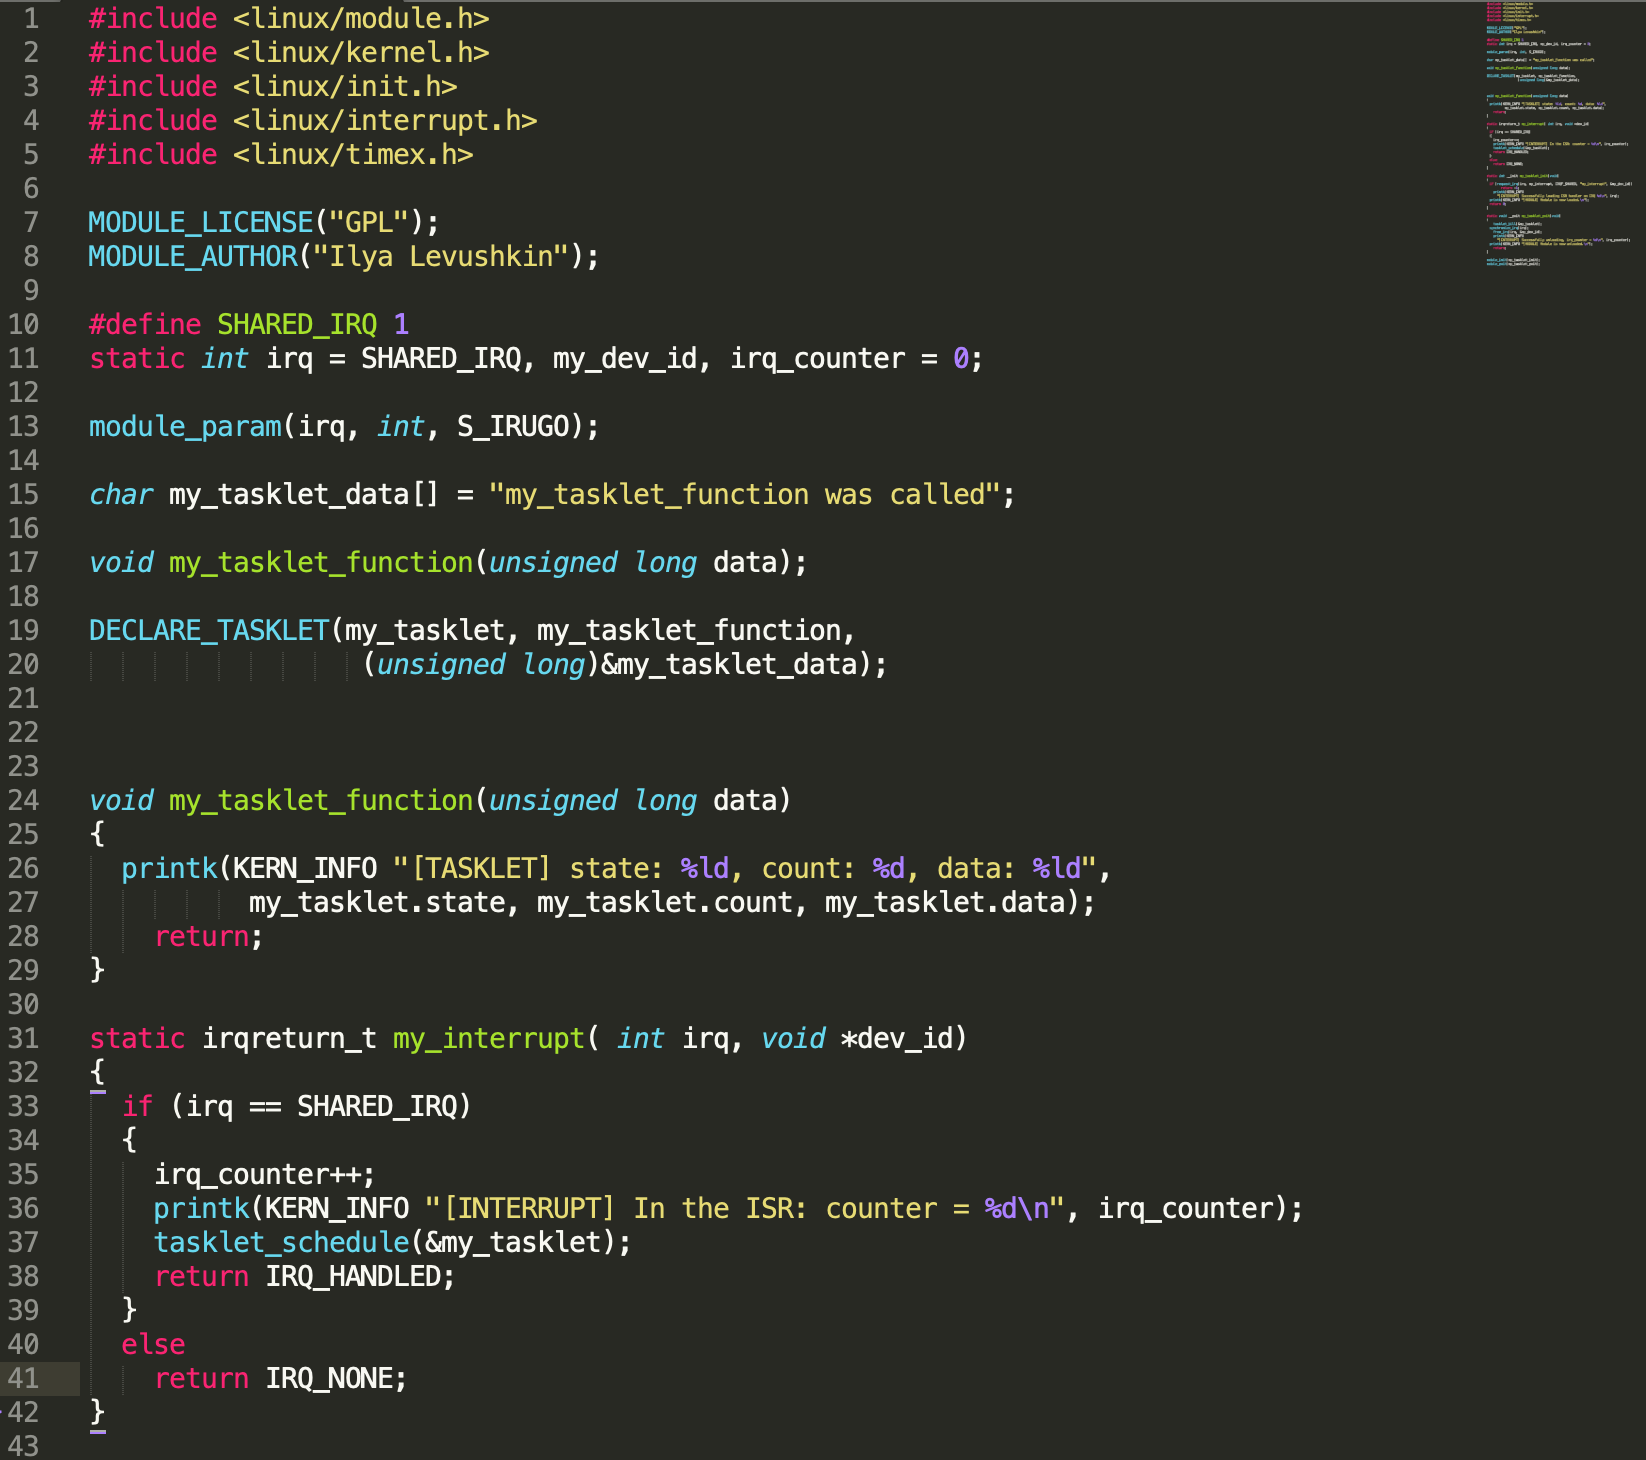
\includegraphics[scale = 0.7]{listing1.png}}
			\label{listing1}
		\end{center}
	\end{figure}

	\newpage

	\begin{figure}[h!]
		\begin{center}
			{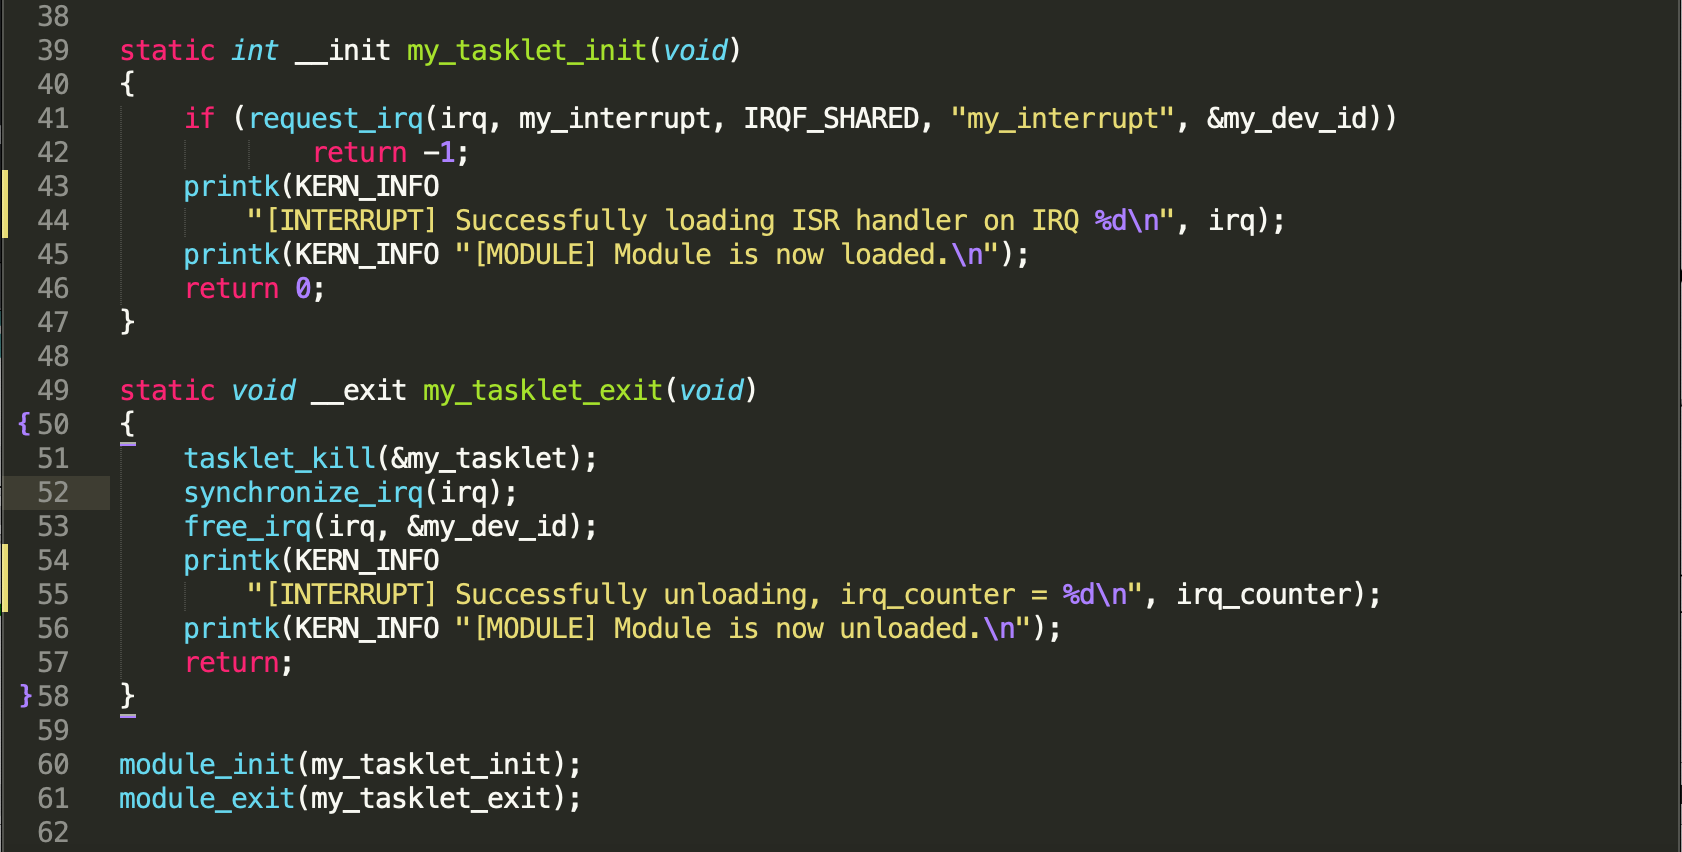
\includegraphics[scale = 0.7]{listing2.png}}
			\label{listing2}
		\end{center}
	\end{figure}

	\newpage
	
	\section*{Демонстрация работы программы}
	
	Загрузка модуля ядра <<tasklet>> с параметром irq = 1 (номер прерывания) и последние 50 сообщений, выведенных модулями ядра (на рисунке показаны последние 17).
	
	\begin{figure}[h!]
		\begin{center}
			{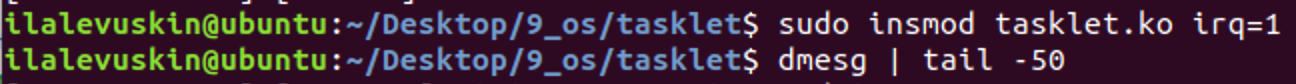
\includegraphics[scale = 0.7]{1.png}}
			\label{1}
		\end{center}
	\end{figure}

	\begin{figure}[h!]
		\begin{center}
			{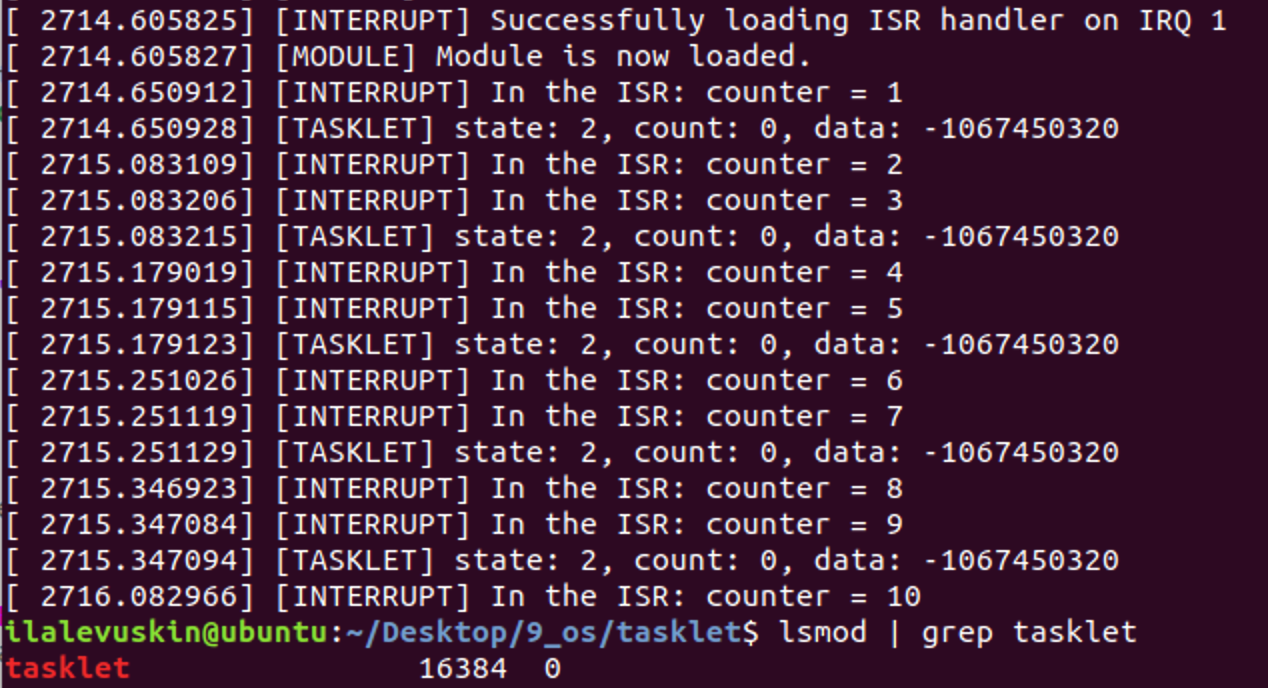
\includegraphics[scale = 0.7]{2.png}}
			\label{2}
		\end{center}
	\end{figure}
	
	Вывод списка загруженных модулей ядра, чье название содержит строку «tasklet»
	
	\begin{figure}[h!]
		\begin{center}
			{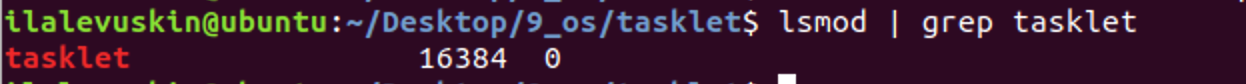
\includegraphics[scale = 0.7]{2.5.png}}
			\label{2.5}
		\end{center}
	\end{figure}

	\newpage
	
	Установленный обработчик 1-ого прерывания в системе:
	
	\begin{figure}[h!]
		\begin{center}
			{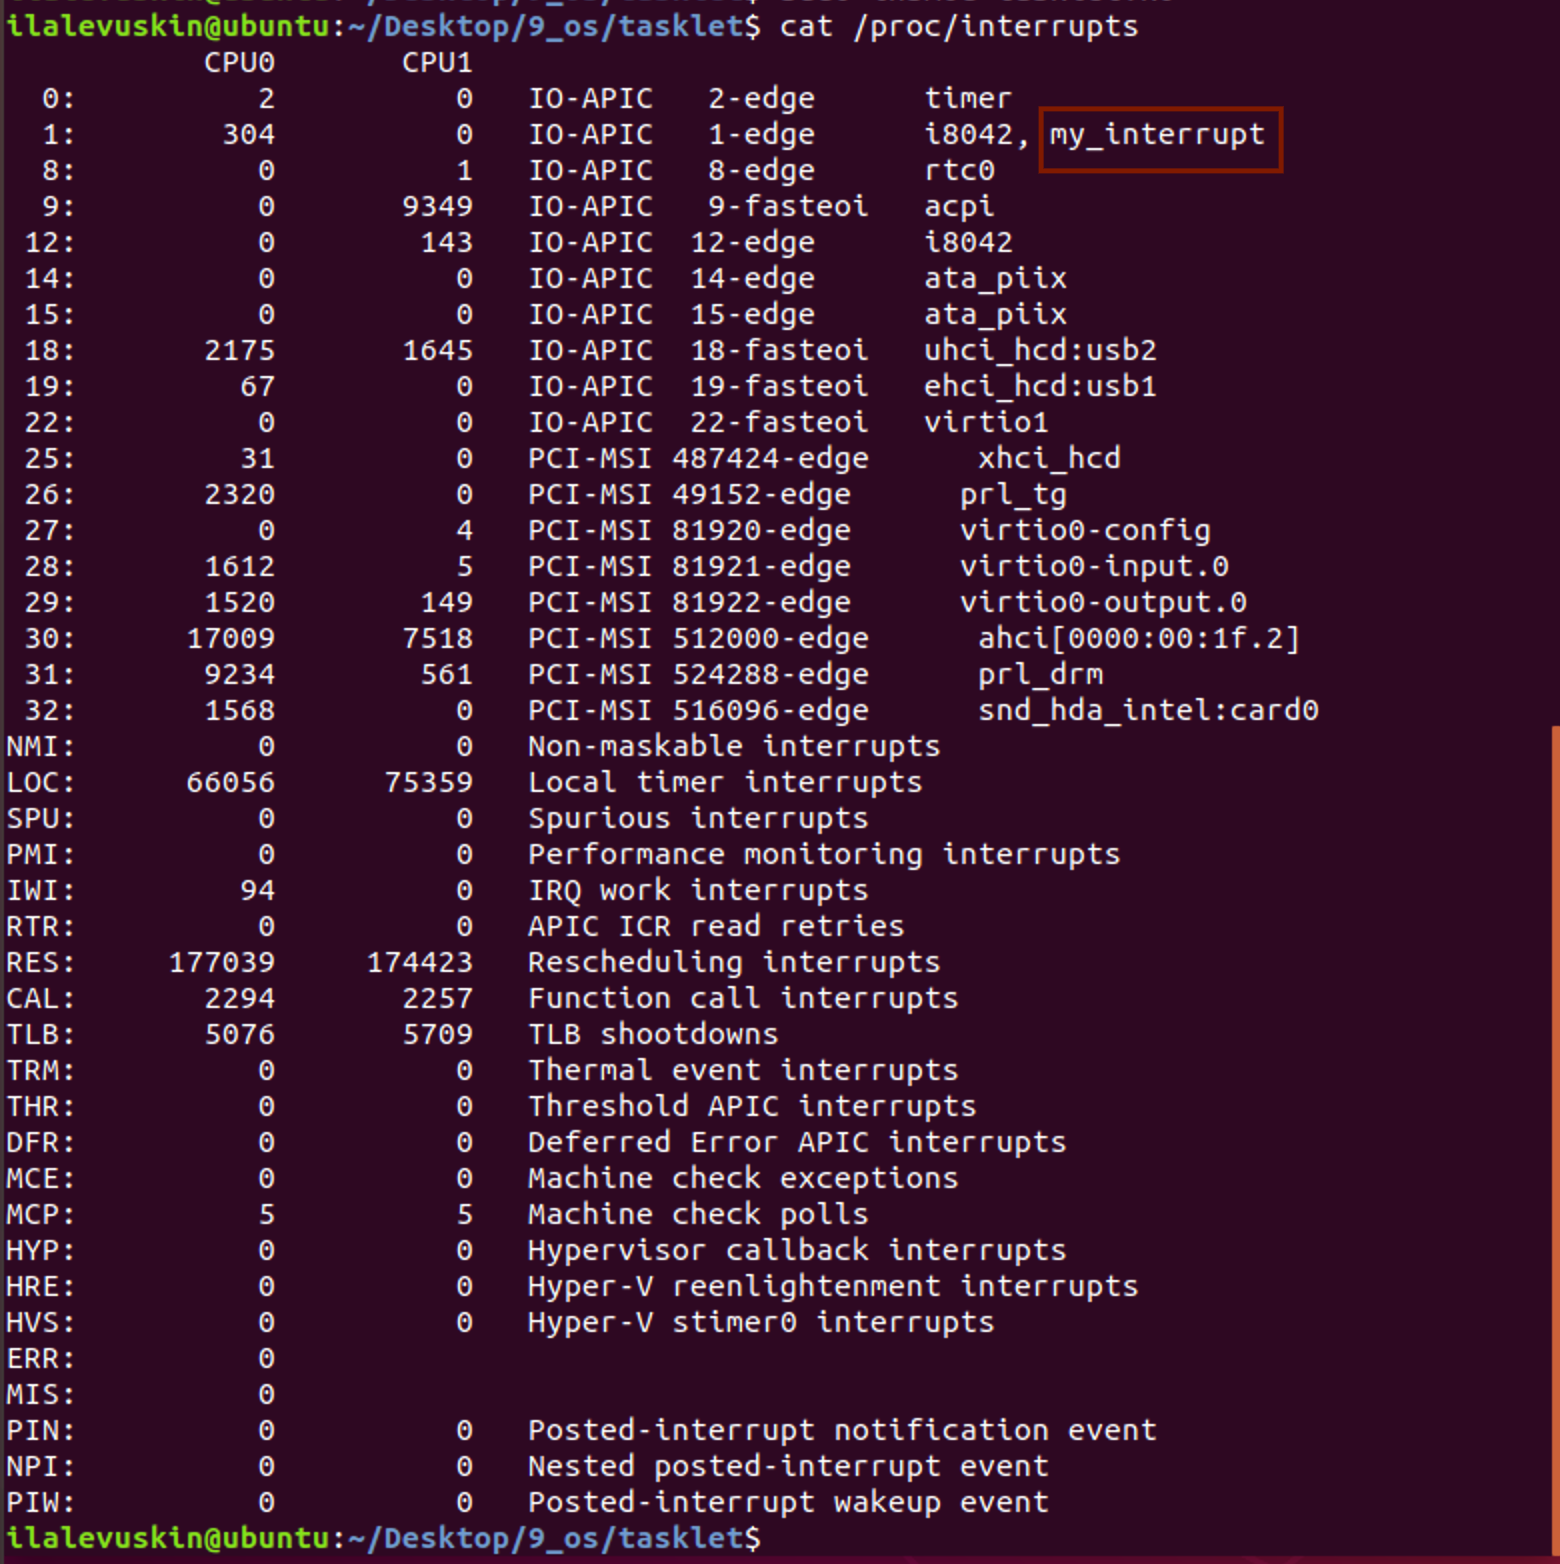
\includegraphics[scale = 0.35]{convert1.png}}
			\label{convert1}
		\end{center}
	\end{figure}
	
	\newpage
	
	Выгрузка модуля ядра <<tasklet>>, последние два сообщения, выведенные модулями ядра.
	
	\begin{figure}[h!]
		\begin{center}
			{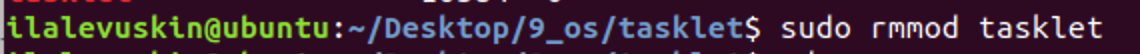
\includegraphics[scale = 0.8]{3.png}}
			\label{3}
		\end{center}
	\end{figure}

	\begin{figure}[h!]
		\begin{center}
			{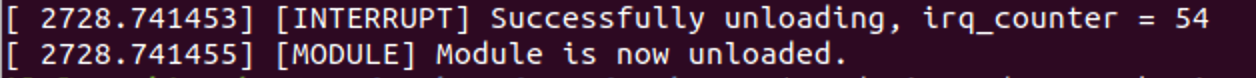
\includegraphics[scale = 0.7]{4.png}}
			\label{4}
		\end{center}
	\end{figure}
	
	Вывод списка загруженных модулей ядра, чье название содержит строку «tasklet»
	
	\begin{figure}[h!]
		\begin{center}
			{
\includegraphics[scale = 0.7]{4.5.png}}
			\label{4.5}
		\end{center}
	\end{figure}
	
	Видно, что модуль ядра <<tasklet>> успешно выгружен.

	\section*{Задание (очередь работ)}
	
	\begin{itemize}
		\item Написать загружаемый модуль ядра, в котором зарегистрировать обработчик аппаратного прерывания с флагом IRQF\_SHARED.
		\item Инициализировать очередь работ.
		\item В обработчике прерывания запланировать очередь работ на выполнение.
		\item Вывести информацию об очереди работ используя, или printk(), или seq\_file interface - <linux/seq\_file.h> (Jonathan Corber: http://lwn.net//Articales//driver-porting/).
	\end{itemize}

	\newpage

	\section*{Листинг кода программы}
	
	\begin{figure}[h!]
		\begin{center}
			{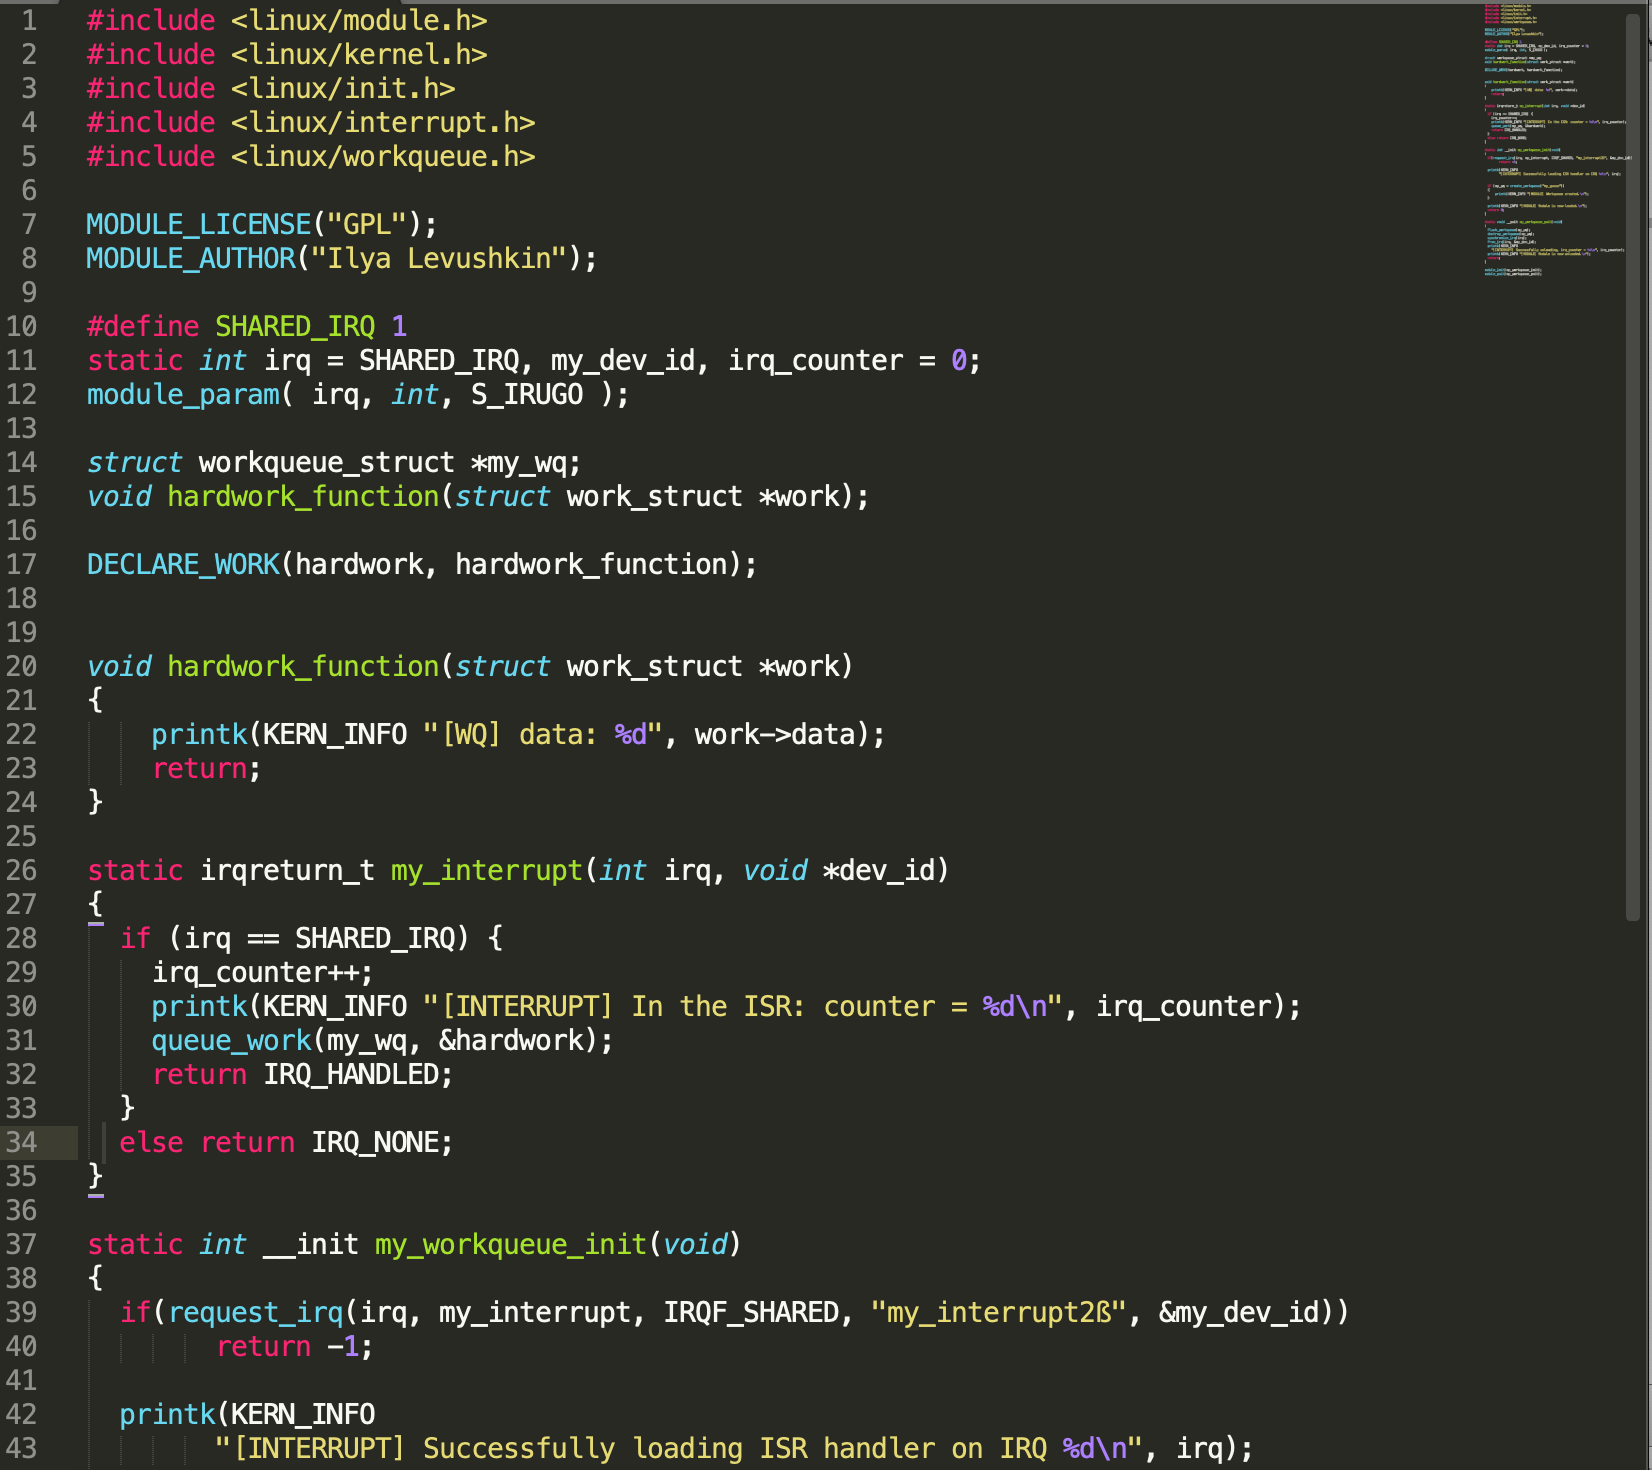
\includegraphics[scale = 0.7]{listing3.png}}
			\label{listing3}
		\end{center}
	\end{figure}

	\newpage

	\begin{figure}[h!]
		\begin{center}
			{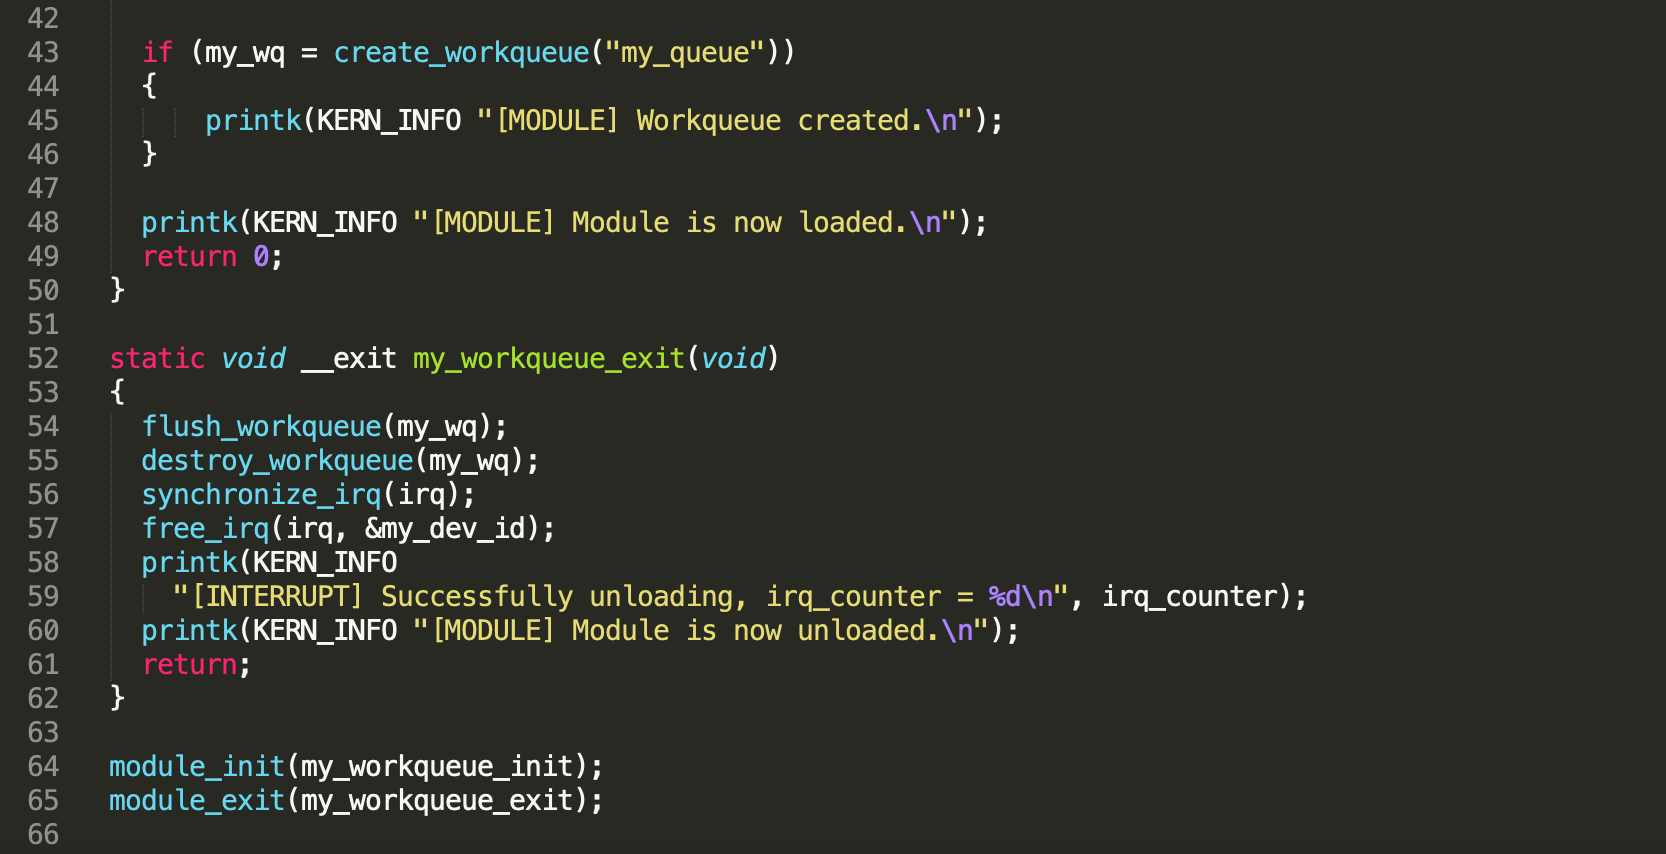
\includegraphics[scale = 0.7]{listing4.png}}
			\label{listing4}
		\end{center}
	\end{figure}
	
	\newpage
	
	\section*{Демонстрация работы программы}
	
	Загрузка модуля ядра <<queue>> с параметром irq = 1 (номер прерывания) и последние 50 сообщений, выведенных модулями ядра (на рисунке показаны последние 30).
	
	\begin{figure}[h!]
		\begin{center}
			{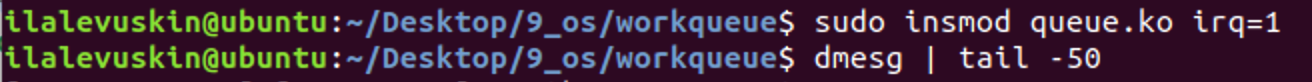
\includegraphics[scale = 0.7]{5.png}}
			\label{5}
		\end{center}
	\end{figure}
	
	\begin{figure}[h!]
		\begin{center}
			{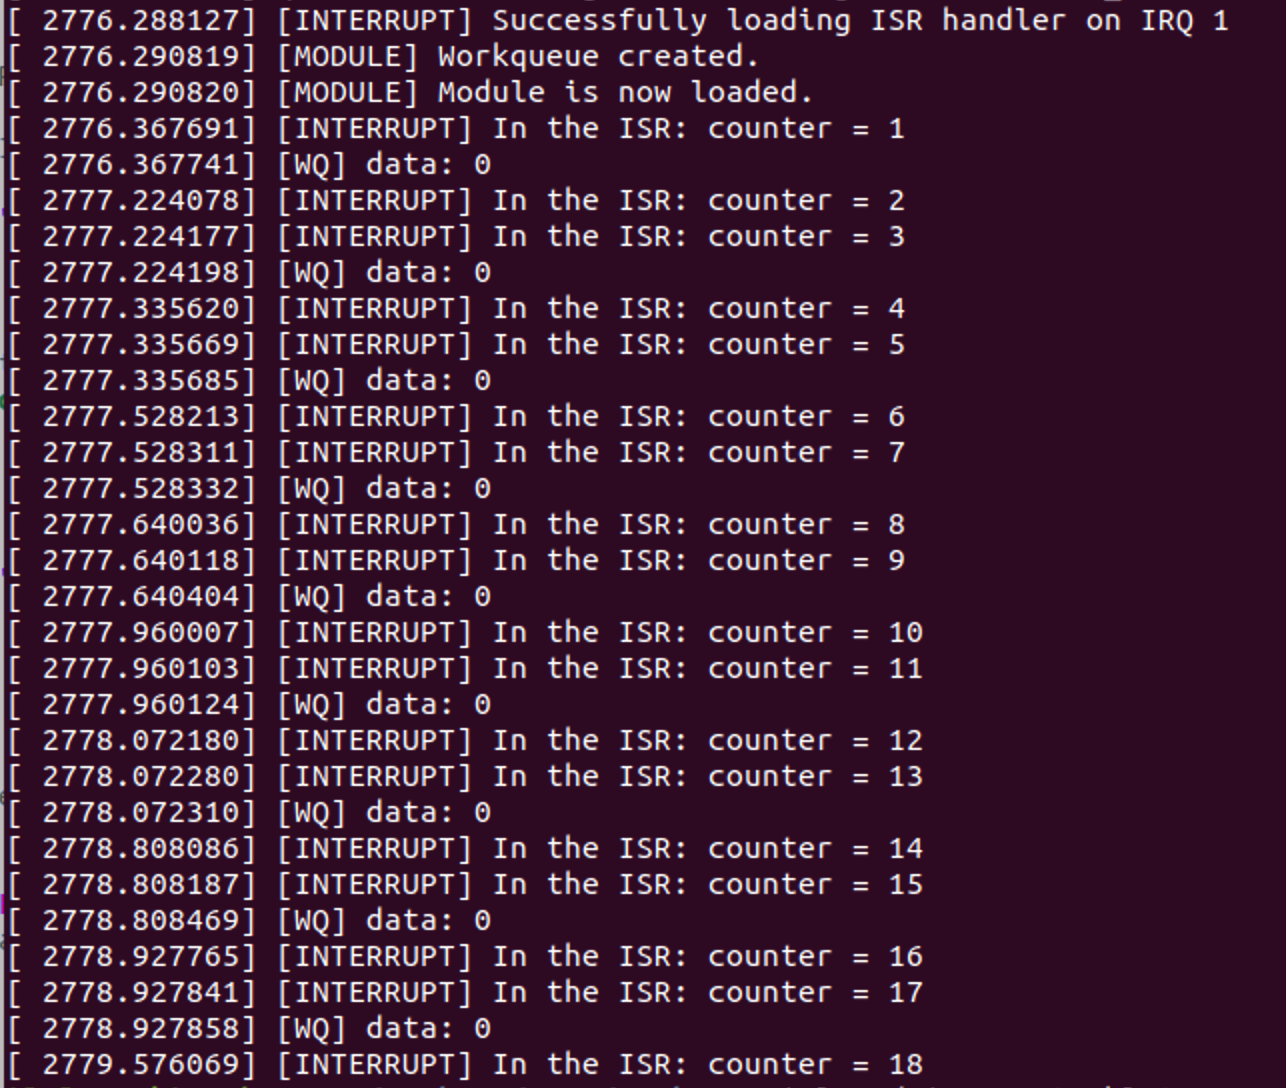
\includegraphics[scale = 0.7]{6.png}}
			\label{6}
		\end{center}
	\end{figure}

	\newpage

	Вывод списка загруженных модулей ядра, чье название содержит строку «queue»
	
	\begin{figure}[h!]
		\begin{center}
			{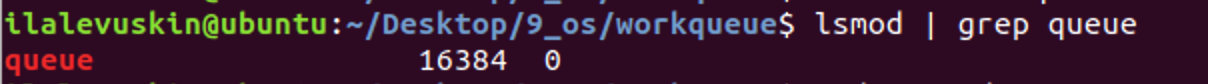
\includegraphics[scale = 0.7]{6.5.png}}
			\label{6.5}
		\end{center}
	\end{figure}
	
	Установленный обработчик 1-ого прерывания в системе:
	
	\begin{figure}[h!]
		\begin{center}
			{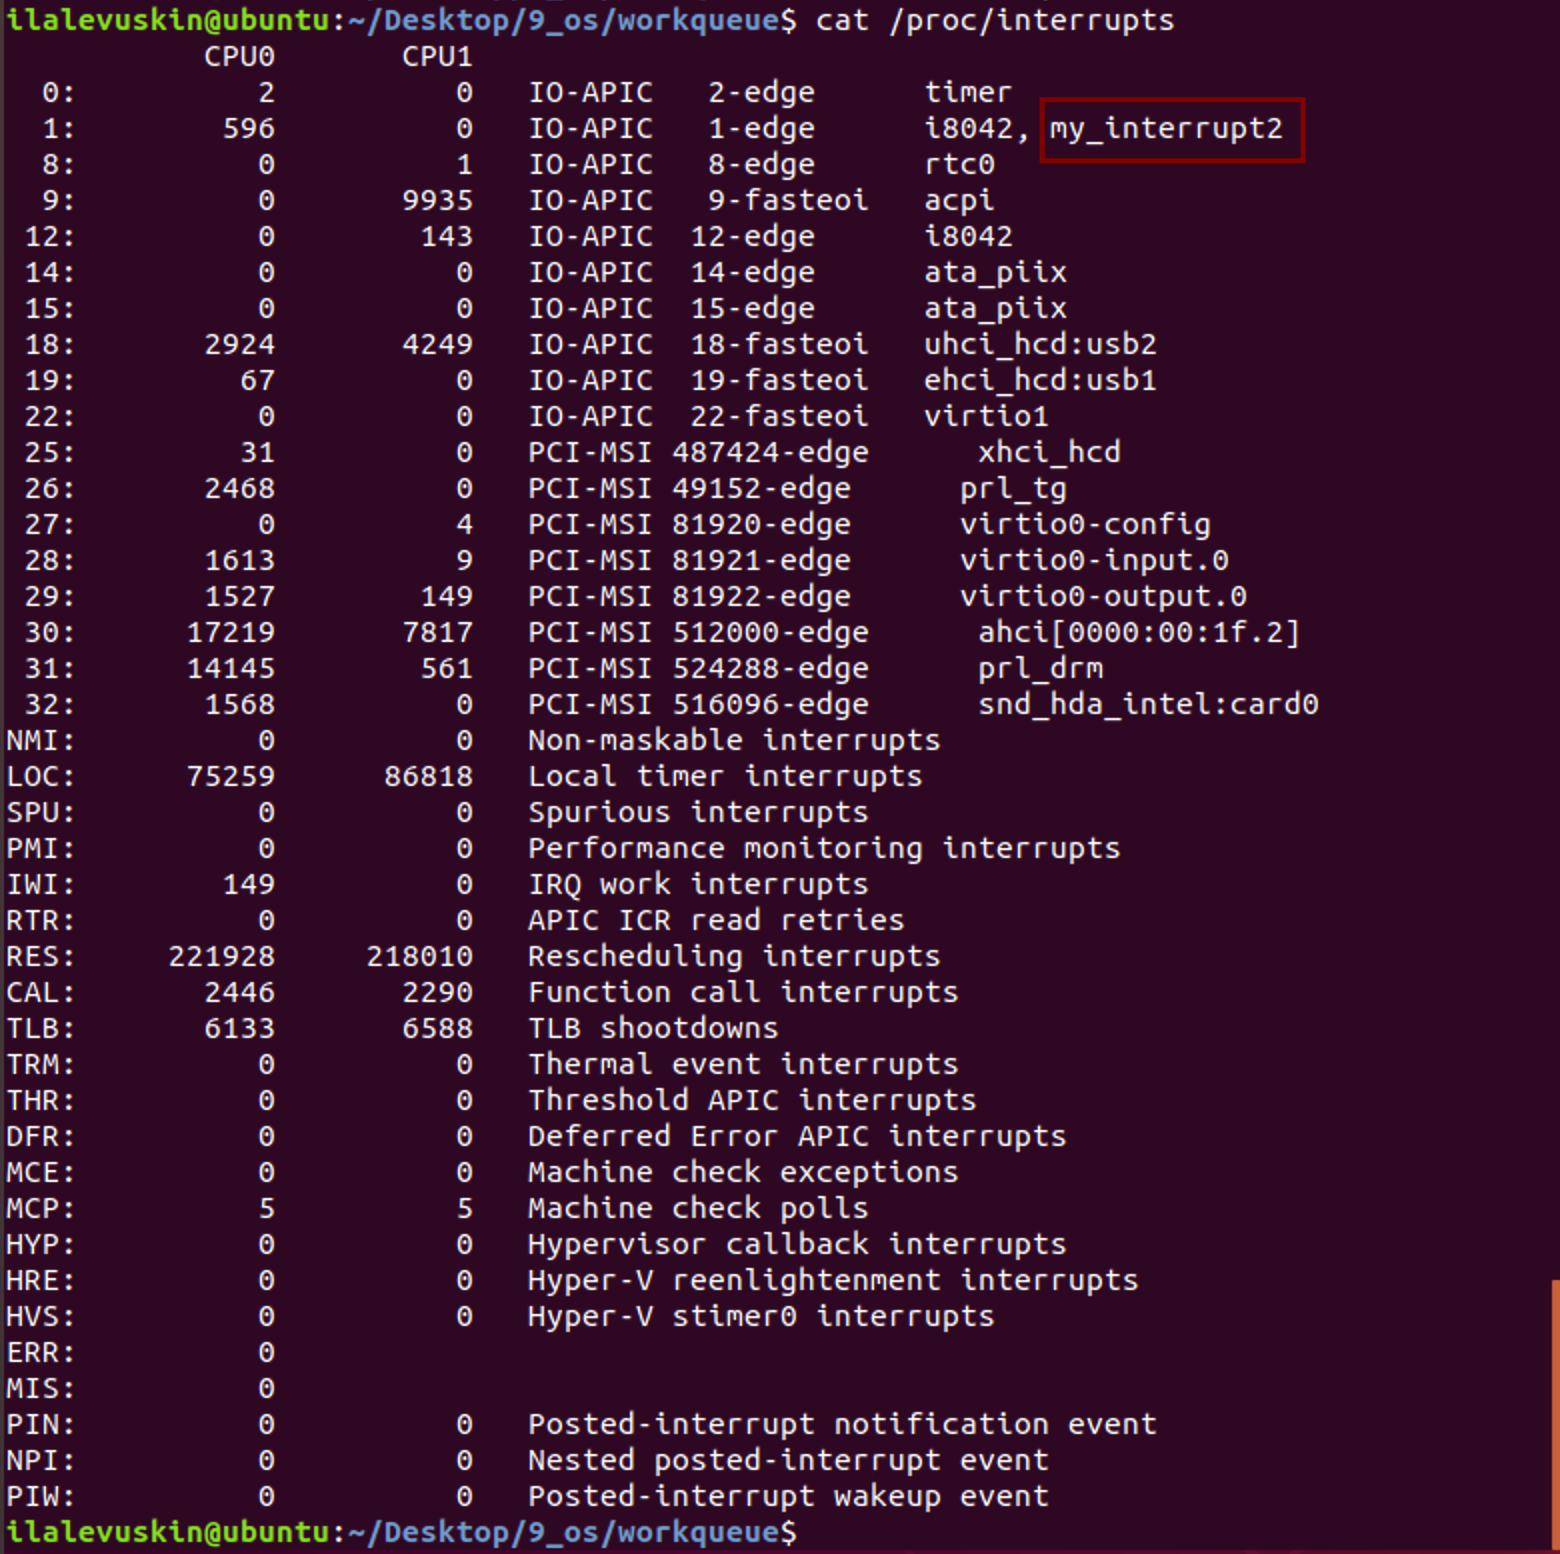
\includegraphics[scale = 0.35]{convert2.png}}
			\label{convert2}
		\end{center}
	\end{figure}
	
	\newpage
	
	Выгрузка модуля ядра <<queue>>, последние два сообщения, выведенные модулями ядра.
	
	\begin{figure}[h!]
		\begin{center}
			{
\includegraphics[scale = 0.8]{7.png}}
			\label{7}
		\end{center}
	\end{figure}
	
	\begin{figure}[h!]
		\begin{center}
			{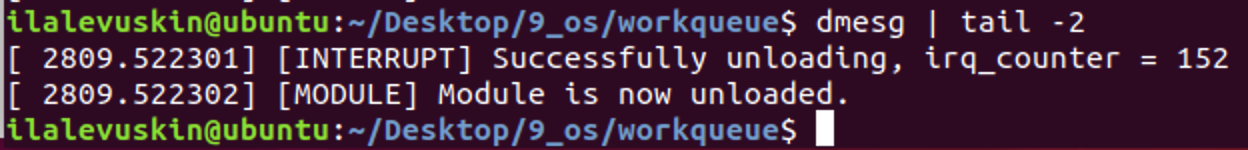
\includegraphics[scale = 0.7]{8.png}}
			\label{8}
		\end{center}
	\end{figure}

	Вывод списка загруженных модулей ядра, чье название содержит строку «queue»
	
	\begin{figure}[h!]
		\begin{center}
			{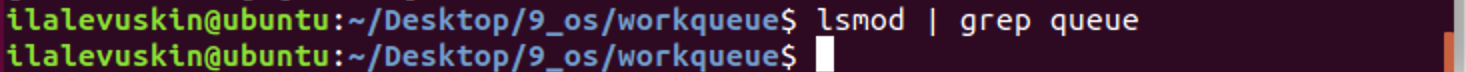
\includegraphics[scale = 0.7]{8.5.png}}
			\label{8}
		\end{center}
	\end{figure}
	
	Видно, что модуль ядра <<queue>> успешно выгружен.
	
	
\end{document}